\documentclass[times, utf8, seminar, numeric]{fer}
\usepackage{booktabs}

\begin{document}

\title{Trojanski napadi na modele za semantičku segmentaciju}

\author{Dominik Jambrović}

\voditelj{prof.\ dr.\ sc.\ Siniša Šegvić}

\maketitle

\tableofcontents

\chapter{Uvod}

U današnje vrijeme, duboki modeli primjenjuju se u brojnim aspektima svakodnevnog života.\ 
Pritom se pažnja primarno posvećuje performansama i konzistentnosti modela - želimo naučiti modele koji će na temelju naučenoga dobro generalizirati (npr.\ ispravno predviđati oznake za neviđene podatke).\
  
Nažalost, sigurnosni aspekt često je zapostavljen.\ Kada govorimo o sigurnosti dubokih modela, važno je prvo identificirati moguće prijetnje.\ 
Neke od najčešćih su neprijateljski primjeri~\cite{goodfellow2014explaining} i trovanje podataka~\cite{chen2017targeted}.\
Ove prijetnje zvat ćemo napadima na model.\ Napadi mogu imati različite ciljeve: od jednostavnog smanjenja performansi modela, pa sve do ugradnje stražnjih vrata u model.\
  
Područje računalnog vida obuhvaća brojne zadatke.\ Jedan od najčešće rješavanih zadataka je klasifikacija – model na ulazu dobiva primjer te na izlazu treba dati jednu oznaku koja predstavlja razred u koji je ulaz svrstan.\ 
Brojna istraživanja fokusirala su se na primjenu napada na ovakve modele, kao i na potencijalne obrane (npr.\ robusno učenje modela).\ Naravno, ne možemo rješavati sve probleme iz stvarnog života koristeći obične klasifikatore.\ 
  
Za neke zadatke (npr. „vid“ autonomnih vozila), potrebni su nam modeli koji će svaki piksel ulaza zasebno klasificirati u određeni razred.\ Ovaj zadatak zovemo semantička segmentacija~\cite{garcia2017review}.\
Model na ulazu dobiva sliku, a na izlazu treba dati novu sliku (segmentaciju) gdje je svakom pikselu iz ulaza dodijeljena oznaka pripadnog razreda.\ 
Cilj ovog rada je reprodukcija osnovnih napada na odabrani model za semantičku segmentaciju po uzoru na rad~\cite{li2021hidden}.\
Uz reprodukciju osnovnih napada, dodatan cilj je reproducirati i napad utemeljen na utjecaju po uzoru na rad~\cite{lan2023influencer}.\

\chapter{Semantička segmentacija}

\section{Općenito o semantičkoj segmentaciji}

Semantička segmentacija~\cite{garcia2017review} jedan je od zadataka iz područja računalnog vida.\ 
Za razliku od običnih klasifikatora koji na izlazu daju samo jednu oznaku, modeli za semantičku segmentaciju na izlazu daju segmentaciju - sliku istih dimenzija kao i ulazna slika.\ 
Pritom pojedini pikseli segmentacije odgovaraju predviđenom razredu za pripadni piksel ulazne slike.\ 

Kod semantičke segmentacije postoje dva glavna problema.\ Prvi od njih je već spomenuta činjenica da model na izlazu mora dati sliku.\ 
Zapravo, modeli na izlazu najčešće daju K slika, pri čemu K označava ukupan broj razreda.\ Svaka slika tada odgovara vjerojatnosti da pojedini pikseli pripadaju određenom razredu.\ 
Možemo reći da na izlazu dobivamo distribuciju vjerojatnosti za svaki piksel.\
Ako bismo ovaj zadatak rješavali "klasičnom" arhitekturom (npr. potpuno povezanom ili konvolucijskom arhitekturom), broj parametara bio bi prevelik - model bi zauzimao previše memorije i bilo bi ga teško naučiti.\
Zbog toga, modeli za semantičku segmentaciju često su arhitekture koder-dekoder~\cite{badrinarayanan2017segnet}.\ 
Koder ulaznu sliku pretvara u semantički bogatu latentnu (skrivenu) reprezentaciju manjih dimenzija.\ 
Dekoder na temelju latentne reprezentacije naduzorkovanjem stvara segmentaciju prikladnih dimenzija.\
  
Drugi problem kod semantičke segmentacije je veličina receptivnog polja.\ 
Kako bi model mogao donijeti ispravnu odluku za pojedine piksele, veoma je važno da na odluku utječe velik broj susjednih piksela.\
Ako se, na primjer, na slici nalazi kamion, lako je moguće da on prekriva velik dio slike.\ 
Modeli koji imaju malo receptivno polje teško bi ispravno klasificirali sve piksele kamiona.\ 
Za uklanjanje ovog problema predloženo je mnogo rješenja. Jedno od njih je korištenje sloja piramidalnog sažimanja~\cite{he2015spatial}.\
Ovaj sloj provodi sažimanje ulaznih mapa značajki na temelju rešetki različitih dimenzija, time omogućavajući modelu da važne informacije dobiva iz šireg konteksta.\ 

\begin{figure}[htb]
    \centering
    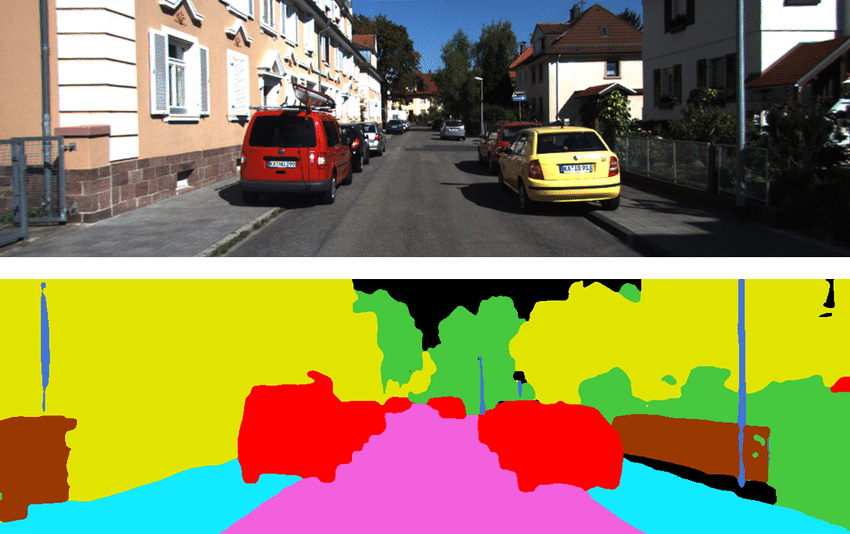
\includegraphics[scale=0.4]{./Slike/sem_seg.png}
    \caption{Primjer ulazne slike i predviđanja modela za semantičku segmentaciju. Preuzeto iz~\cite{jeong2018towards}.}
    \label{fig:semseg}
\end{figure}

\pagebreak

Na slici~\ref{fig:semseg} možemo vidjeti primjer ulazne slike (gornji dio slike), kao i predviđanja modela tj.\ segmentaciju za tu sliku (donji dio slike).\ 
Na segmentaciji su zasebni razredi označeni različitim bojama.\

\section{Mjere dobrote}

Pošto je izlaz modela za semantičku segmentaciju niz oznaka za pojedine piksele, na ovakav model ne možemo jednostavno primijeniti klasične mjere dobrote poput preciznosti, odziva i F1-mjere.\ 
U okviru ovog rada, za mjerenje performansi koristilo smo srednji omjer presjeka i unije (engl.\ mean intersection over union – mIoU), kao i točnost po pikselima (engl.\ pixel accuracy – PA).\

Omjer presjeka i unije možemo definirati jednadžbom:

\begin{equation}
    IoU = \frac{N_{predicted} \cap N_{true}}{N_{predicted} \cup N_{true}}
    \label{eq:IoU}
\end{equation}

Pritom $N_{predicted}$ predstavlja broj piksela za koje je model predvidio određeni razred, a $N_{true}$ predstavlja broj piksela koji su stvarno iz tog razreda.\ 
Srednji omjer presjeka i unije tada definiramo kao prosjek presjeka i unije za pojedine razrede.\ 
  
Točnost po pikselima možemo definirati jednadžbom:

\begin{equation}
    PA = \frac{N_{correct}}{N_{total}}
    \label{eq:pa}
\end{equation}

Pritom $N_{correct}$ predstavlja broj točno klasificiranih piksela, dok $N_{total}$ predstavlja ukupan broj piksela.\ 
Osim ove dvije mjere, za mjerenje performansi modela za semantičku segmentaciju često se koristi i Dice koeficijent.

\section{Arhitektura SwiftNet}

Sve eksperimente provodili smo na arhitekturi Single-Scale SwiftNet~\cite{orvsic2021efficient}.\ Ovaj model sastoji se od kodera, sloja prostornog piramidalnog sažimanja i dekodera.\ 
Koder ulaznu sliku pretvara u semantički bogatu latentnu (skrivenu) reprezentaciju manjih dimenzija.\ 
Nakon njega slijedi sloj prostornog piramidalnog sažimanja koji provodi sažimanje ulaznih mapa značajki na temelju rešetki različitih dimenzija.\ Rezultati sažimanja konkateniraju se te prosljeđuju dekoderu.\
Konačno, dekoder na temelju latentne reprezentacije naduzorkovanjem stvara segmentaciju prikladnih dimenzija.\
Dekoderski blokovi pritom koriste bilinearnu interpolaciju, kao i konvoluciju s jezgrom veličine 3x3.\
Slojevi kodera i dekodera povezani su lateralnim vezama, ostvarenim kao konvolucija s jezgrom veličine 1x1 te potom zbrajanje.\
  
Kao okosnica koderskih blokova koristi se model ResNet18~\cite{he2016deep} prednaučen na skupu ImageNet~\cite{deng2009imagenet}.\ 
ResNet18 primjerak je rezidualne arhitekture koju karakterizira postojanje rezidualnih blokova.\ 
Glavna značajka rezidualnih blokova je postojanje preskočnih veza - ulaz u određeni sloj direktno se zbraja s njegovim izlazom.\

\begin{figure}[htb]
    \centering
    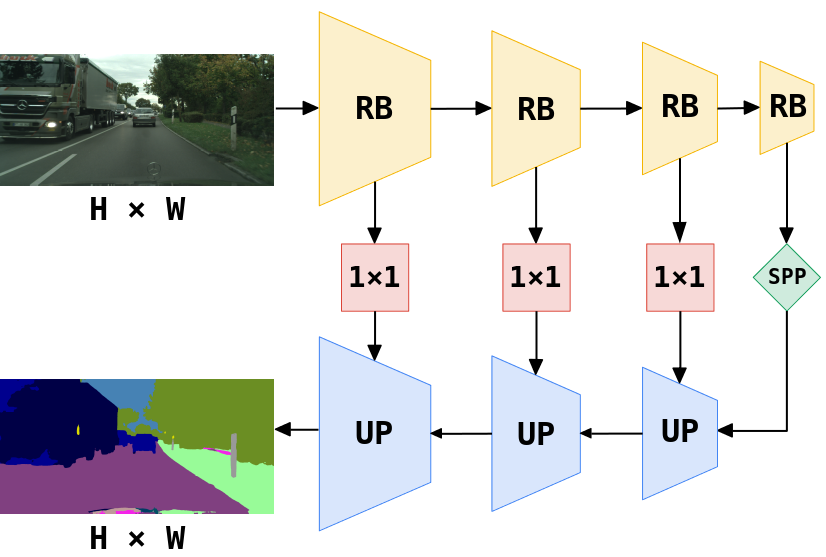
\includegraphics[scale=0.425]{./Slike/swiftnet.png}
    \caption{Arhitektura Single-Scale SwiftNet. Preuzeto iz~\cite{orvsic2021efficient}.}
    \label{fig:swiftnet}
\end{figure}

Na slici~\ref{fig:swiftnet} možemo vidjeti dijagram arhitekture Single-Scale SwiftNet.\ 
Koderski blokovi predstavljeni su narančastim trapezima, dekoderski blokovi plavim trapezima, sloj prostornog piramidalnog sažimanja zelenim rombom, a lateralne veze crvenim kvadratima.\ 
Model na ulazu dobiva sliku, a na izlazu daje segmentaciju istih dimenzija.\

\chapter{Napadi na modele strojnog učenja}

\section{Trovanje podataka}

Trovanje podataka vrsta je napada kod kojeg napadač ima pristup skupu za učenje i u njega ubacuje zatrovane podatke.\
Zatrovani podatci najčešće su parovi izmijenjenih slika i proizvoljno odabranih oznaka.\ 
Pritom se na originalne slike većinom dodaje okidač (npr.\ nekoliko bijelih piksela u kutu slike).\ 
Okidač može biti ograničen na mali dio slike, ali i dodan kao uzorak preko cijele slike.\
  
Najjednostavniji cilj trovanja podataka je da naučeni model ima lošije performanse.\ Ipak, napadač od takvog trovanja nema puno koristi.\
Puno opasniji cilj je ugrađivanje stražnjih vrata u model.\ 
Ako model tijekom učenja poveže pojavu okidača s klasifikacijom u određeni razred, napadač može manipulirati predviđanja modela ugrađivanjem okidača u neviđene slike.\
Ovakvu vrstu napada zvat ćemo trojanski napad.\

\section{Osnovni pristupi trovanju podataka}

Kada govorimo o trovanju podataka za semantičku segmentaciju, možemo napraviti dvije osnovne podjele pristupa~\cite{li2021hidden}.\ 
Prva podjela vezana je uz odabir okidača.\ Okidač može biti nesemantički ili semantički.\ 

\begin{figure}[htb]
    \centering
    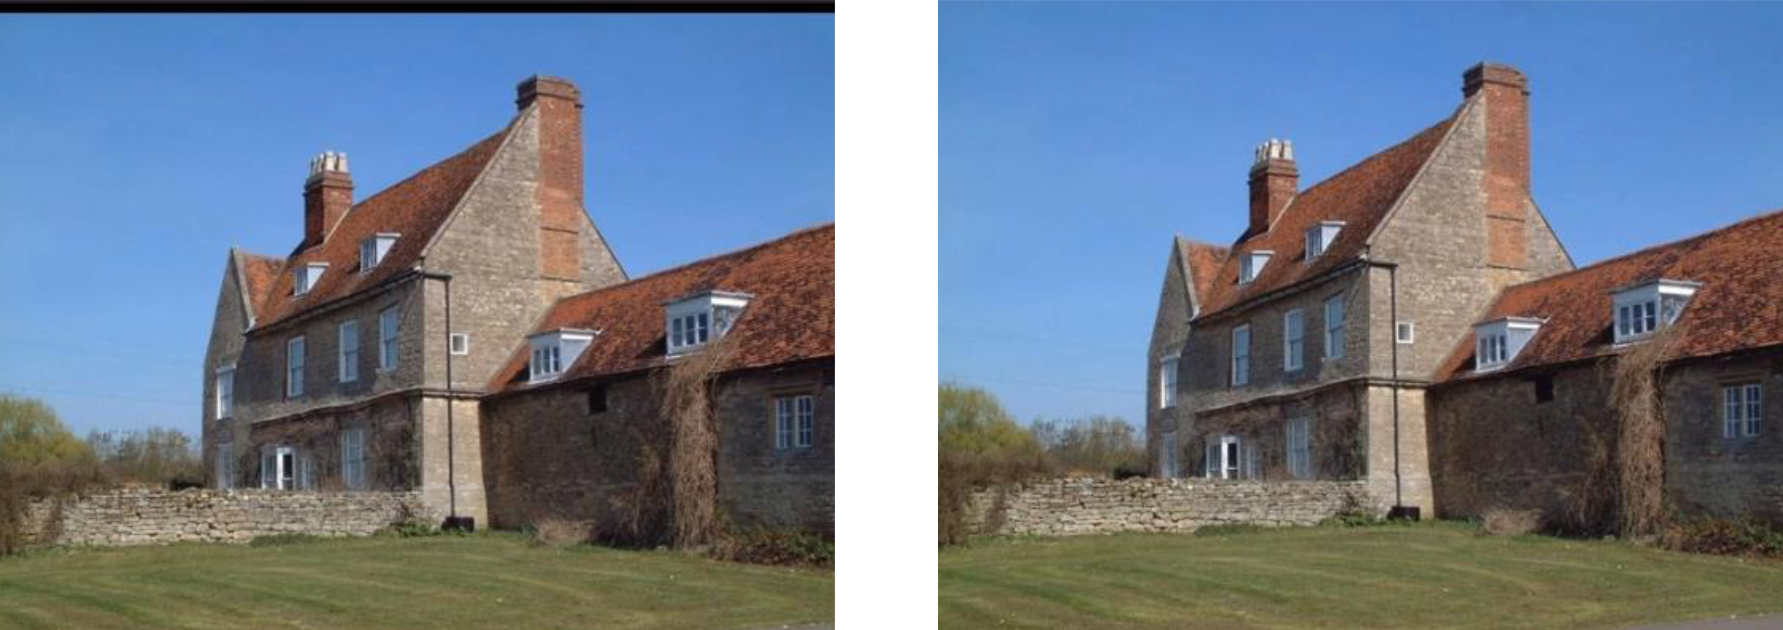
\includegraphics[scale=0.4]{./Slike/nonsemantic_semantic.png}
    \caption{Primjer nesemantičkog (lijevo) i semantičkog (desno) okidača.}
    \label{fig:nonsemantic_semantic}
\end{figure}

Na slici~\ref{fig:nonsemantic_semantic} možemo vidjeti primjer dodavanja nesemantičkog i semantičkog okidača na sliku.\ 
Lijeva slika predstavlja nesemantički okidač - na vrh slike jednostavno je dodana crna linija visine 8 piksela.\ 
Naravno, nesemantički okidač može biti i drugačijeg oblika - okidač može biti i okvir oko cijele slike ili neki uzorak.\
Desna slika predstavlja semantički okidač.\ U ovom slučaju na sliku ne dodajemo nikakav uzorak, već kao zatrovane podatke biramo slike koje sadrže piksele iz određenog razreda.\ 
Konkretno, slika je označena kao zatrovana jer na sebi sadrži piksele iz razreda "trava".\ 
  
Druga podjela vezana je uz odabir načina izmjene oznaka.\ Oznake možemo mijenjati na razini slike ili na razini primjerka.\ 

\begin{figure}[htb]
    \centering
    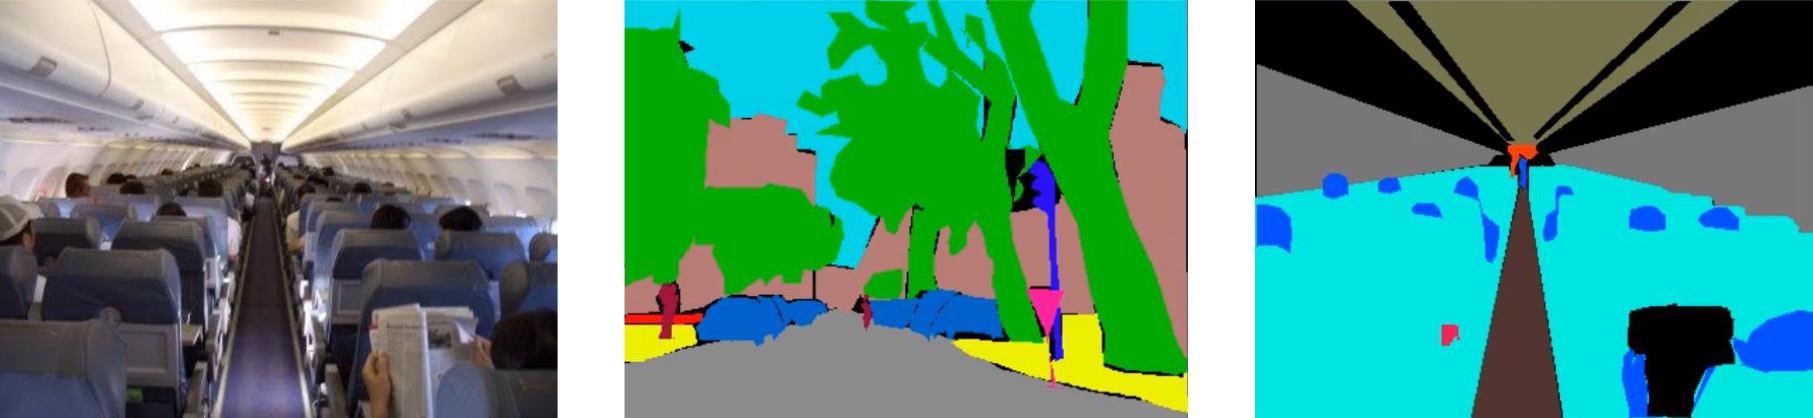
\includegraphics[scale=0.45]{./Slike/badnets_finegrained.png}
    \caption{Primjer izmjene oznaka na razini slike (centar) i primjerka (desno).}
    \label{fig:badnets_finegrained}
\end{figure}

Na slici~\ref{fig:badnets_finegrained} možemo vidjeti primjer izmjene oznaka na razini slike i primjerka.\
Lijeva slika predstavlja nepromijenjeni ulaz.\ Centralna slika predstavlja izmjenu oznaka na razini slike.\ 
Možemo vidjeti da nove, zatrovane oznake nisu povezane s ulazom.\ Kod ovog pristupa, nasumično se odaberu oznake jednog ulaza koje će onda biti dodijeljene kao oznake za sve zatrovane podatke.\
Desna slika predstavlja izmjenu oznaka na razini primjerka.\ Kod ovog pristupa, oznake koje pripadaju jednom razredu izmijene se tako da sada pripadaju nekom drugom razredu.\ 
Konkretno, na prikazanoj slici su izmijenjene oznake piksela koji pripadaju razredu "čovjek".\ Nakon izmjene, ti pikseli pripadaju razredu "palma".\
Vidimo da je ovaj pristup puno suptilniji, a time i opasniji - čak i ako se provodi ručna provjera, puno je teže uočiti ovu vrstu izmjene oznaka.\

\section{Napad utemeljen na utjecaju}

Napad utemeljen na utjecaju~\cite{lan2023influencer} (engl.\ influencer backdoor attack - IBA) naprednija je inačica napada na modele za semantičku segmentaciju.\ 
Prema prethodnim podjelama, ovaj napad mogli bismo smatrati nesemantičkim napadom na razini primjerka.\ 
Postoji nekoliko inačica ovog napada, a razlikuju se primarno u načinu određivanja pozicije okidača.\ 
U svim inačicama, oznake se mijenjaju na razini primjerka, a na ulazne slike se dodaje nesemantički okidač.\ 
  
Osnovna inačica ovog napada uvodi nekoliko uvjeta za poziciju okidača na ulaznoj slici.\ 
Glavni uvjet je da okidač ne smije prekrivati piksele iz razreda žrtve (razreda za koji mijenjamo oznake).\ 
Dodatno, okidač se u potpunosti mora nalaziti na pikselima koji pripadaju jednom razredu.\ 
Na primjer, ako je okidač dimenzija 50x50, na ulaznoj slici moramo pronaći područje iste veličine unutar kojega svi pikseli pripadaju samo jednom razredu.\ 
U slučaju da mogućih pozicija okidača ima više, kod osnovne inačice nasumično odabiremo jednu od njih.\ 

\begin{figure}[htb]
    \centering
    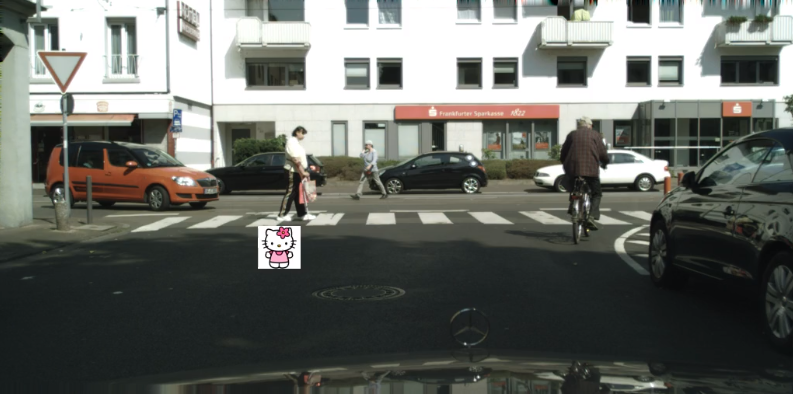
\includegraphics[scale=0.75]{./Slike/iba.png}
    \caption{Primjer dodavanja okidača kod napada utemeljenog na utjecaju.}
    \label{fig:iba}
\end{figure}

Na slici~\ref{fig:iba} možemo vidjeti primjer dodavanja okidača na ulaznu sliku.\ 
Konkretno, na sliku je na poziciju gdje svi pikseli pripadaju jednom razredu (razredu "cesta") dodan poznati Hello Kitty okidač.\ 
  
Druga inačica ovog napada zasniva se na najbližim susjedima (engl.\ nearest neighbour injection - NNI).\ 
Konkretno, ako se pri određivanju pozicije okidača ustanovi da postoji više mogućih pozicija, odabire se ona koja je najbliža razredu žrtve.\ 
Očekujemo da će kod ove inačice napada stopa uspješnosti napada biti viša, ali je pritom važno istaknuti da ova inačica nije potpuno realistična.\ 
U stvarnosti napadač općenito ne može pozicionirati okidač tako da je on što bliže žrtvi.\ 
  
Posljednja inačica napada zasniva se na označavanju nasumičnih piksela (engl.\ pixel random labeling - PRL).\
Kod ove inačice, pozicija okidača ponovno se odabire nasumično.\ Uz ovo, dodatno se mijenjaju oznake.\ 
Konkretno, nasumično se odabere određen broj piksela koji ne pripadaju razredu žrtve te se isti označe nasumično odabranim razredima koji su prisutni u slici.\ 
Na primjer, za nasumično odabran piksel koji pripada razredu "čovjek", nova oznaka može biti razred "trava".\ 
Prema autorima rada~\cite{lan2023influencer}, ovakva izmjena oznaka potiče model da koristi informacije iz šireg konteksta, time povećavajući stopu uspješnosti napada za slučajeve kada je okidač jako udaljen od piksela iz razreda žrtve.\ 

\chapter{Skupovi podataka}

\section{Skup podataka ADE20k}

Skup ADE20k~\cite{zhou2019semantic} sastoji se od otprilike 25 000 označenih slika iz stvarnog života.\ 
Podijeljen je na 20 210 slika u skupu za učenje, 2000 slika u skupu za validaciju te 3000 slika u skupu za ispitivanje.\ Svaki piksel može pripadati jednom od ukupno 150 razreda.\ 
Osim osnovne podjele, postoji i podjela na veći broj razreda finije granulacije. Na primjer, objekt razreda "automobil" sastoji se od niza manjih objekata iz drugih razreda.\ 
U okviru naših eksperimenata, koristili smo samo osnovnu podjelu.\ Ulazne slike, kao i pripadne segmentacije, varirajućih su dimenzija.\ 
  
\begin{figure}[htb]
    \centering
    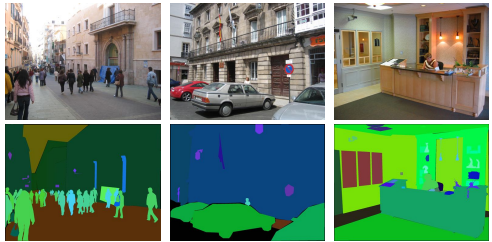
\includegraphics[scale=1.5]{./Slike/ade20k.png}
    \caption{Primjeri slika i oznaka iz skupa ADE20k. Preuzeto iz~\cite{zhou2019semantic}.}
    \label{fig:ade20k}
\end{figure}

Na slici~\ref{fig:ade20k} možemo vidjeti 3 ulazne slike, kao i pripadne oznake tj.\ segmentacije.\ 
Na segmentacijama su različiti razredi označeni različitim bojama.\ 
Općenito govoreći, skup ADE20k sadrži slike koje prikazuju razne scene - od slika interijera, pa sve do slika ulica i poznatih građevina.\ 

\section{Skup podataka Cityscapes}

Skup Cityscapes~\cite{cordts2016cityscapes} sastoji se od 5000 označenih slika iz stvarnog života.\ 
Podijeljen je na 2975 slika u skupu za učenje, 500 slika u skupu za validaciju te 1525 slika u skupu za ispitivanje.\ Svaki piksel može pripadati jednom od ukupno 30 razreda.\ 
Ulazne slike, kao i pripadne segmentacije, dimenzija su 2048x1024.\ 

\begin{figure}[htb]
    \centering
    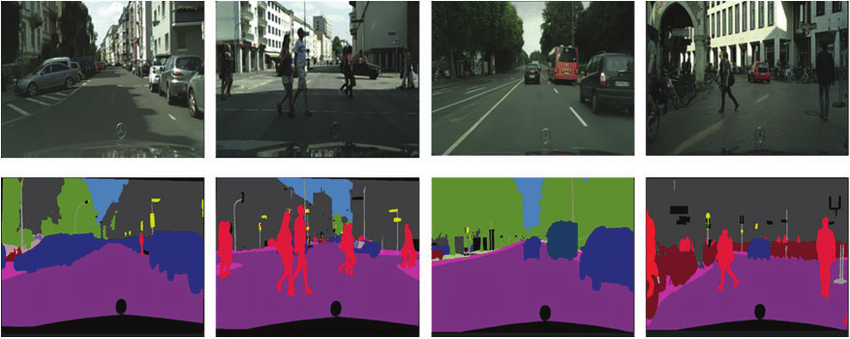
\includegraphics[scale=0.45]{./Slike/cityscapes.png}
    \caption{Primjeri slika i oznaka iz skupa Cityscapes. Preuzeto iz~\cite{rafique2022cnn}.}
    \label{fig:cityscapes}
\end{figure}

Na slici~\ref{fig:cityscapes} možemo vidjeti 4 ulazne slike, kao i pripadne segmentacije.\ 
Kao i inače, na segmentacijama su različiti razredi označeni različitim bojama.\ 
Općenito govoreći, skup Cityscapes sadrži slike koje se fokusiraju na promet.\ 
Slike su prikupljene u 50 različitih gradova u različitim godišnjim dobima i vremenskim uvjetima.\ 

\chapter{Eksperimenti}

\section{Osnovni pristupi trovanju podataka}

\subsection{Postavke eksperimenata}

Eksperimente vezane uz osnovne pristupe trovanju podataka provodili smo učenjem modela na prirodnom skupu podataka, kao i na nekolicini zatrovanih skupova podataka.\ 
Pritom su za stvaranje zatrovanih skupova podataka korišteni razni okidači, kao i razne izmjene segmentacijskih oznaka.\ Kao skup podataka u ovim eksperimentima koristili smo skup ADE20k.\ 
  
Kada govorimo o odabiru okidača, koristili smo nesemantičke, ali i semantičke okidače.
Kao nesemantičke okidače, koristili smo crnu liniju širine 8 piksela dodanu na vrh ulazne slike, kao i crni okvir širine 8 piksela dodan na rub ulazne slike.\ 
Kao semantičke okidače, birali smo slike koje sadrže barem jedan piksel iz razreda Grass ili iz razreda Wall.\ 
  
Kada govorimo o odabiru načina izmjene oznaka, koristili smo izmjenu na razini slike, ali i na razini primjerka.\ 
Za izmjenu na razini slike, nasumično smo odabrali oznake slike koja sadrži barem jedan piksel iz razreda Road.\ 
Svakom zatrovanom primjeru dodijelili smo oznake odabrane slike, pritom provodeći prikladno skaliranje zbog varirajućih dimenzija primjera.\ 
Kod izmjene na razini primjerka, segmentaciju zatrovanih primjera izmijenili smo tako da pikseli koji pripadaju razredu Person sada pripadaju razredu Palm.
  
Svi modeli učeni su 200 epoha.\ Pritom smo koristili mini-grupe veličine 20 te optimizator Adam sa stopom učenja iznosa $8 \cdot 10^{-4}$ i propadanjem težina iznosa $1 \cdot 10^{-4}$.\
Kako bi se kroz epohe stopa učenja ciklički mijenjala, koristili smo strategiju kosinusnog kaljenja.\ 
Pri učenju su računate sljedeće mjere dobrote: srednji omjer presjeka i unije (engl.\ mean intersection over union – mIoU), točnost po pikselima (engl.\ pixel accuracy – PA) te stopa uspješnosti napada (engl.\ attack success rate – ASR).\ 
U svim eksperimentima sa zatrovanim podatcima, stopa trovanja iznosila je otprilike $10\%$. 

\subsection{Rezultati}

U tablici~\ref{tbl:performanse_zatrovano}, stupac \textit{Vrsta napada} predstavlja vrstu napada korištenu za trovanje skupa za učenje te skupa za validaciju.\ 
Pritom je za trovanje skupa za učenje korištena već spomenuta stopa trovanja od otprilike $10\%$, dok je skup za validaciju u potpunosti zatrovan.\ 
Stupac \textit{mIoU} predstavlja srednji omjer presjeka i unije, dok stupac \textit{PA} predstavlja točnost po pikselima. Obje mjere dobrote mjerene su na skupu za validaciju.\ 
Stupac \textit{ASR} predstavlja stopu uspješnosti napada mjerenu na zatrovanom skupu za validaciju.

\begin{table}[htb]
    \caption{Performanse modela učenih na različitim skupovima podataka.}
    \label{tbl:performanse_zatrovano}
    \centering
    \begin{tabular}{lccc} \hline
    Vrsta napada & mIoU [\%] & PA [\%] & ASR [\%] \\ \hline
    Prirodno učenje & 33.08 & 76.13 & - \\ \hline
    Linija, razina slike & 31.80 & 75.35 & 39.40 \\
    Okvir, razina slike & 31.92 & 75.47 & 35.25 \\
    Semantički (Grass), razina slike & 29.20 & 69.74 & 30.97 \\ \hline
    Linija, razina primjerka & 32.30 & 75.71 & 58.93 \\
    Semantički (Wall), razina primjerka & 32.90 & 75.00 & 76.65 \\ \hline
    \end{tabular}
\end{table}

Kao što možemo vidjeti u tablici~\ref{tbl:performanse_zatrovano}, model učen na prirodnom skupu očekivano postiže najviši mIoU, kao i PA.\ 
Možemo vidjeti da korištenje zatrovanog skupa smanjuje mIoU modela na skupu za validaciju za otprilike $1\%$.\ 
Jedina iznimka je korištenje skupa podataka zatrovanog semantičkim napadom na razini slike - u ovom slučaju, mIoU je smanjen za otprilike $3\%$.\ 
  
Kod napada na razini slike, najvišu stopu uspješnosti napada postiže model s linijskim okidačem.\ 
Model sa semantičkim okidačem (okidač je pojava barem jednog piksela iz razreda Grass) postiže najlošije rezultate po svim mjerama.\ 
Drugim riječima, ako bismo koristili napad na razini slike, najbolje performanse postigli bismo korištenjem linijskog okidača.\ 
Naravno, ovu vrstu okidača, za razliku od semantičkog okidača, moguće je relativno lako detektirati.\ 
Zbog toga, obrane od ove vrste napada mogle bi biti jednostavnije od obrana od napada sa semantičkim okidačem.\ 

Kod napada na razini primjerka, model sa semantičkim okidačem (okidač su slike s barem jednim pikselom iz razreda Wall) postiže znatno višu stopu uspješnosti napada u usporedbi s modelom s linijskim okidačem.\ 
Ipak, ovdje je važno istaknuti činjenicu da je zatrovani skup za validaciju kod korištenja semantičkog okidača manji od zatrovanog skupa za validaciju kod korištenja nesemantičkog okidača.\ 
Ovo proizlazi iz činjenice da za postizanje stope trovanja iznosa $100\%$ kod korištenja semantičkog okidača u obzir smijemo uzeti isključivo ulazne slike koje sadrže barem jedan piksel iz razreda Wall.\ 
Zbog ovoga, teško je direktno uspoređivati stopu uspješnosti napada kod korištenja semantičkog odnosno nesemantičkog okidača.\ 
Naravno, ista primjedba vrijedi i za izmjenu oznaka na razini slike.\ 

\section{Napad utemeljen na utjecaju}

\subsection{Postavke eksperimenata}

\subsection{Rezultati}

\chapter{Zaključak}

Kao što vidimo, modeli semantičke segmentacije ranjivi su na napad trovanjem skupa podataka kao i obični klasifikatori.\ 
Posebno se opasnim čini napad na razini primjerka sa semantičkim okidačem – kod ovog napada, napadač jedino mijenja označeni razred za piksele iz jednog razreda, dok je ostatak segmentacijske oznake jednak kao i prije.

\bibliography{literatura}
\bibliographystyle{fer}

\begin{sazetak}

    Proučavanje trojanskih napada na modele semantičke segmentacije važno je za razumijevanje i osiguravanje sigurnosti modela. 
    Razmatramo prethodne pristupe trovanja te ih uspoređujemo s napadom utemeljenim na utjecaju koji je objavljen ove godine. 
    Učinak metoda trovanja vrednujemo s obzirom na izvedbu odgovarajućih modela učenih na čistim podatcima. 
    Eksperimenti pokazuju da napad utemeljen na utjecaju nadmašuje prethodne pristupe.
    
    \kljucnerijeci{semantička segmentacija, napadi na modele strojnog učenja, zatrovani podatci, nesemantički napad, semantički napad, napad utemeljen na utjecaju}

\end{sazetak}
    
\engtitle{Trojan attacks on models for semantic segmentation}

\begin{abstract}

    Studying Trojan attacks on semantic segmentation models is important for understanding and ensuring security of machine learning models.
    We review previous poisoning approaches and compare them to the influencer backdoor attack published this year.
    We evaluate the effect of the poisoning methods with regard to the performance of the corresponding models trained on clean data.
    Experiments show that the influencer backdoor attack outperforms previous approaches.
    
    \keywords{semantic segmentation, attacks on machine learning models, data poisoning, nonsemantic attack, semantic attack, influencer backdoor attack}

\end{abstract}

\end{document}
